\documentclass[a4paper]{article}

\usepackage[utf8]{inputenc}

\usepackage{url}
\usepackage[]{hyperref}

\usepackage{caption}

\usepackage{listings}

\usepackage{color}

\usepackage{amsmath}

\usepackage{pythonhighlight}

% *** GRAPHICS RELATED PACKAGES ***
%\usepackage[pdftex]{graphicx}
\usepackage{graphicx}
%\usepackage[dvips]{graphicx}
% to place figures on a fixed position
\usepackage{float}

\usepackage[margin=1in]{geometry}

\title{Traffic analysis study – Queuing Theory I. Home Assignment I.}
\author{Ferenc Nandor Janky - OA8AT9}
\date{}


\begin{document}

\maketitle

\tableofcontents

\section{Introduction}

The goal of the 1st home assignment is to perform a similar traffic analysis study that is presented in \cite{MolnarOnburst} with an arbitrarily chosen time series.
For the analysis a capture file was selected from \url{http://ita.ee.lbl.gov/}. The link to the actual capture file archive is \url{ftp://ita.ee.lbl.gov/traces/dec-pkt-1.tar.Z}. This capture contains 3.3 million packets from 1995. The packets are further filtered into multiple files based on packet types (TCP,UDP,etc.). This analysis deals with \verb!dec-pkt-1.tcp! from the archive mentioned before that is around 62 MBytes ands contains around 2.2 million TCP packets.


\section{Implementation}

The calculation and plotting of the resulting graphs have been implemented in the Python programming language.The software is available on \url{https://github.com/fecjanky/QT_home_assignment/blob/master/ha1/toki1.py}.
For the implementation the following Python libraries have been utilized:

\begin{itemize}
\item \verb!matplotlib! , for plotting various statistical data
\item \verb!numpy! , for effective numerical calculations
\end{itemize}

\section{Results}

\subsection{General metrics}

The values of Peak-to-Mean Ration (PMR), Squared Coefficient of Variation (SCV) and Skewness (S) of the inter-arrival data set  -- that was calculated from the arrival time series using the code in Listing~\ref{lst:interarr} --
 were the following:

 \begin{align*} 
& PMR = & 250.4374 & \\
& SCV = & 2.2048  & \\
& S   = & 6.2460 &
\end{align*} 

 
\begin{lstlisting}[style=mypython,caption={The functions used for calculating IDI and IDC},label={lst:interarr}]
def calc_interarrivals(arrivals):
    if len(arrivals) < 2:
        return None
    return np.subtract(np.array(arrivals[1:]), arrivals[0:-2])
\end{lstlisting}


\subsection{Intensity graph}

Figure~\ref{fig:intensity} shows the intensity graph of the analyzed capture. The intensity was aggregated using a 1 second basis based on the arrival times.

\begin{figure}[H]
    \centering
    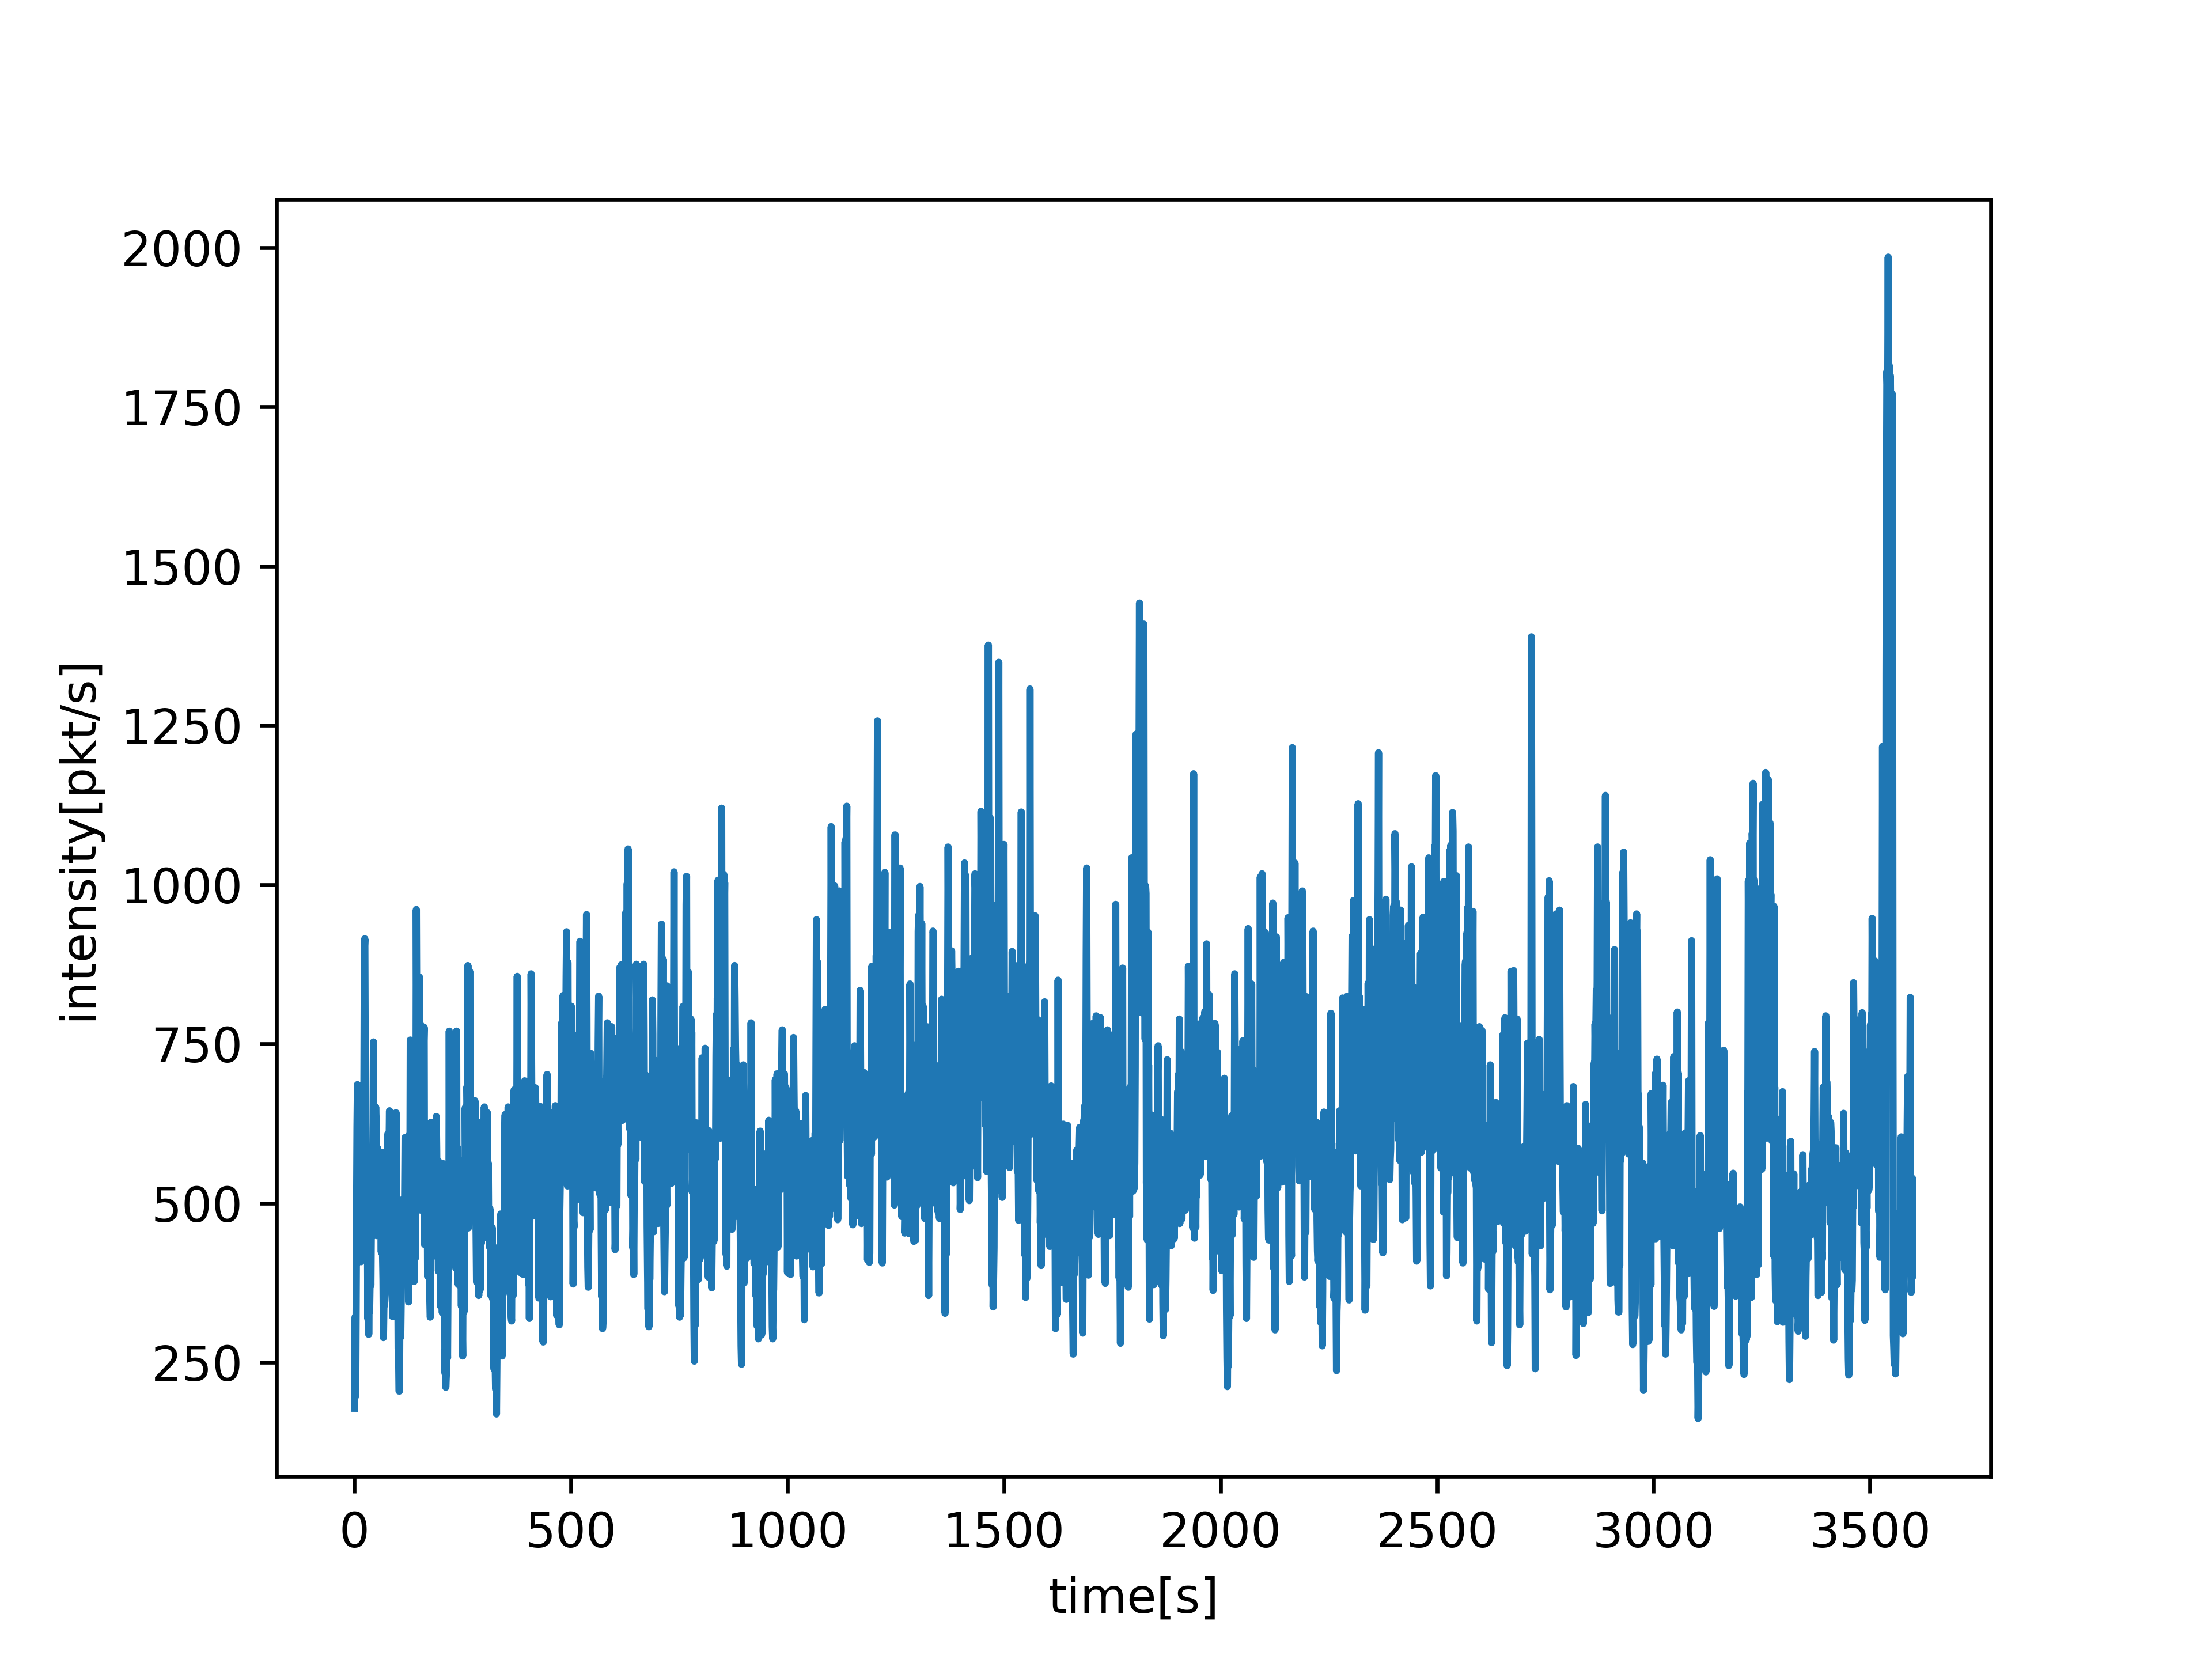
\includegraphics[width=0.9\textwidth]{figures/intensity.png}
    \caption{Intensity graph of the analyzed packet capture}
    \label{fig:intensity}
\end{figure}

\subsection{Inter-arrival KDE}

Figure~\ref{fig:interarrival} shows the kernel density estimation of the packet inter-arrival times.

\begin{figure}[H]
    \centering
    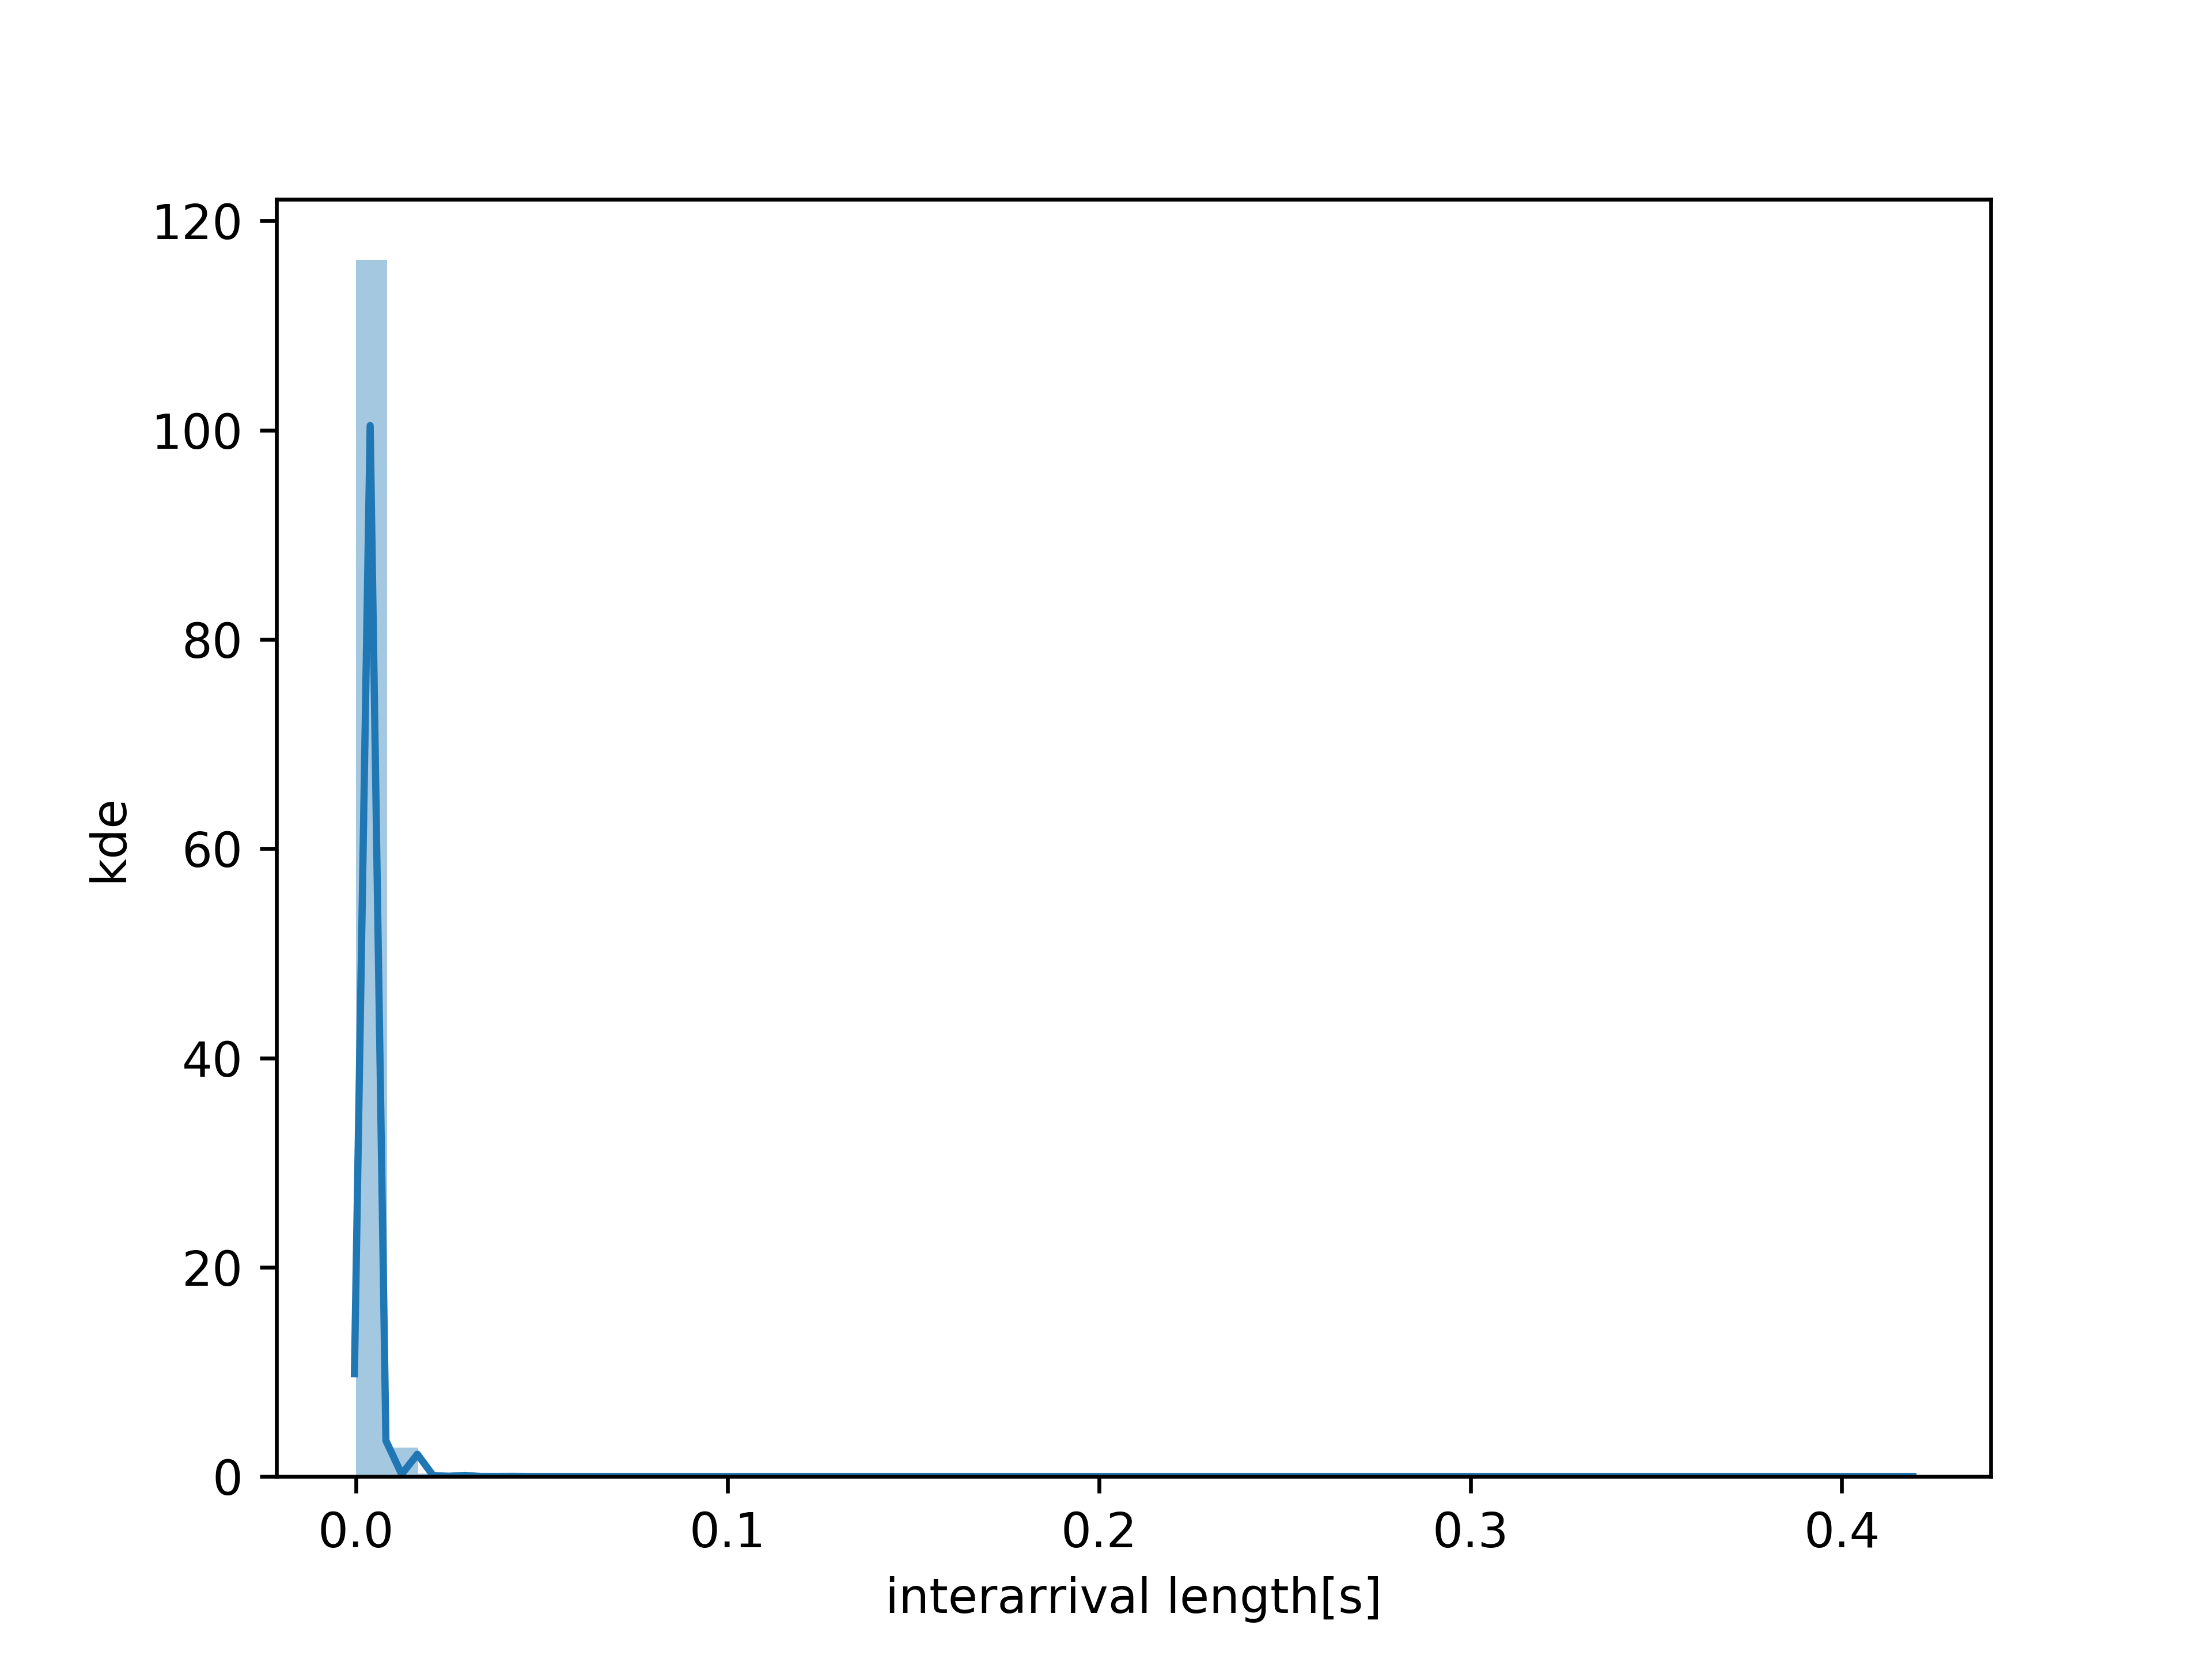
\includegraphics[width=0.9\textwidth]{figures/interarrival.png}
    \caption{KDE graph of the inter-arrival times}
    \label{fig:interarrival}
\end{figure}

\subsection{Packet count and inter-arrival auto-correlation}

The following two Figures \ref{fig:countcorr} and \ref{fig:interarrcorr} shows the auto-correlation of the intensity and inter-arrival data as a function of lag.
Figure~\ref{fig:countcorr} shows signs of auto-correlation levels that could be an indicator of traffic bursts. Figure~\ref{fig:interarrcorr} shows slight auto-correlation also.

\begin{figure}[H]
    \centering
    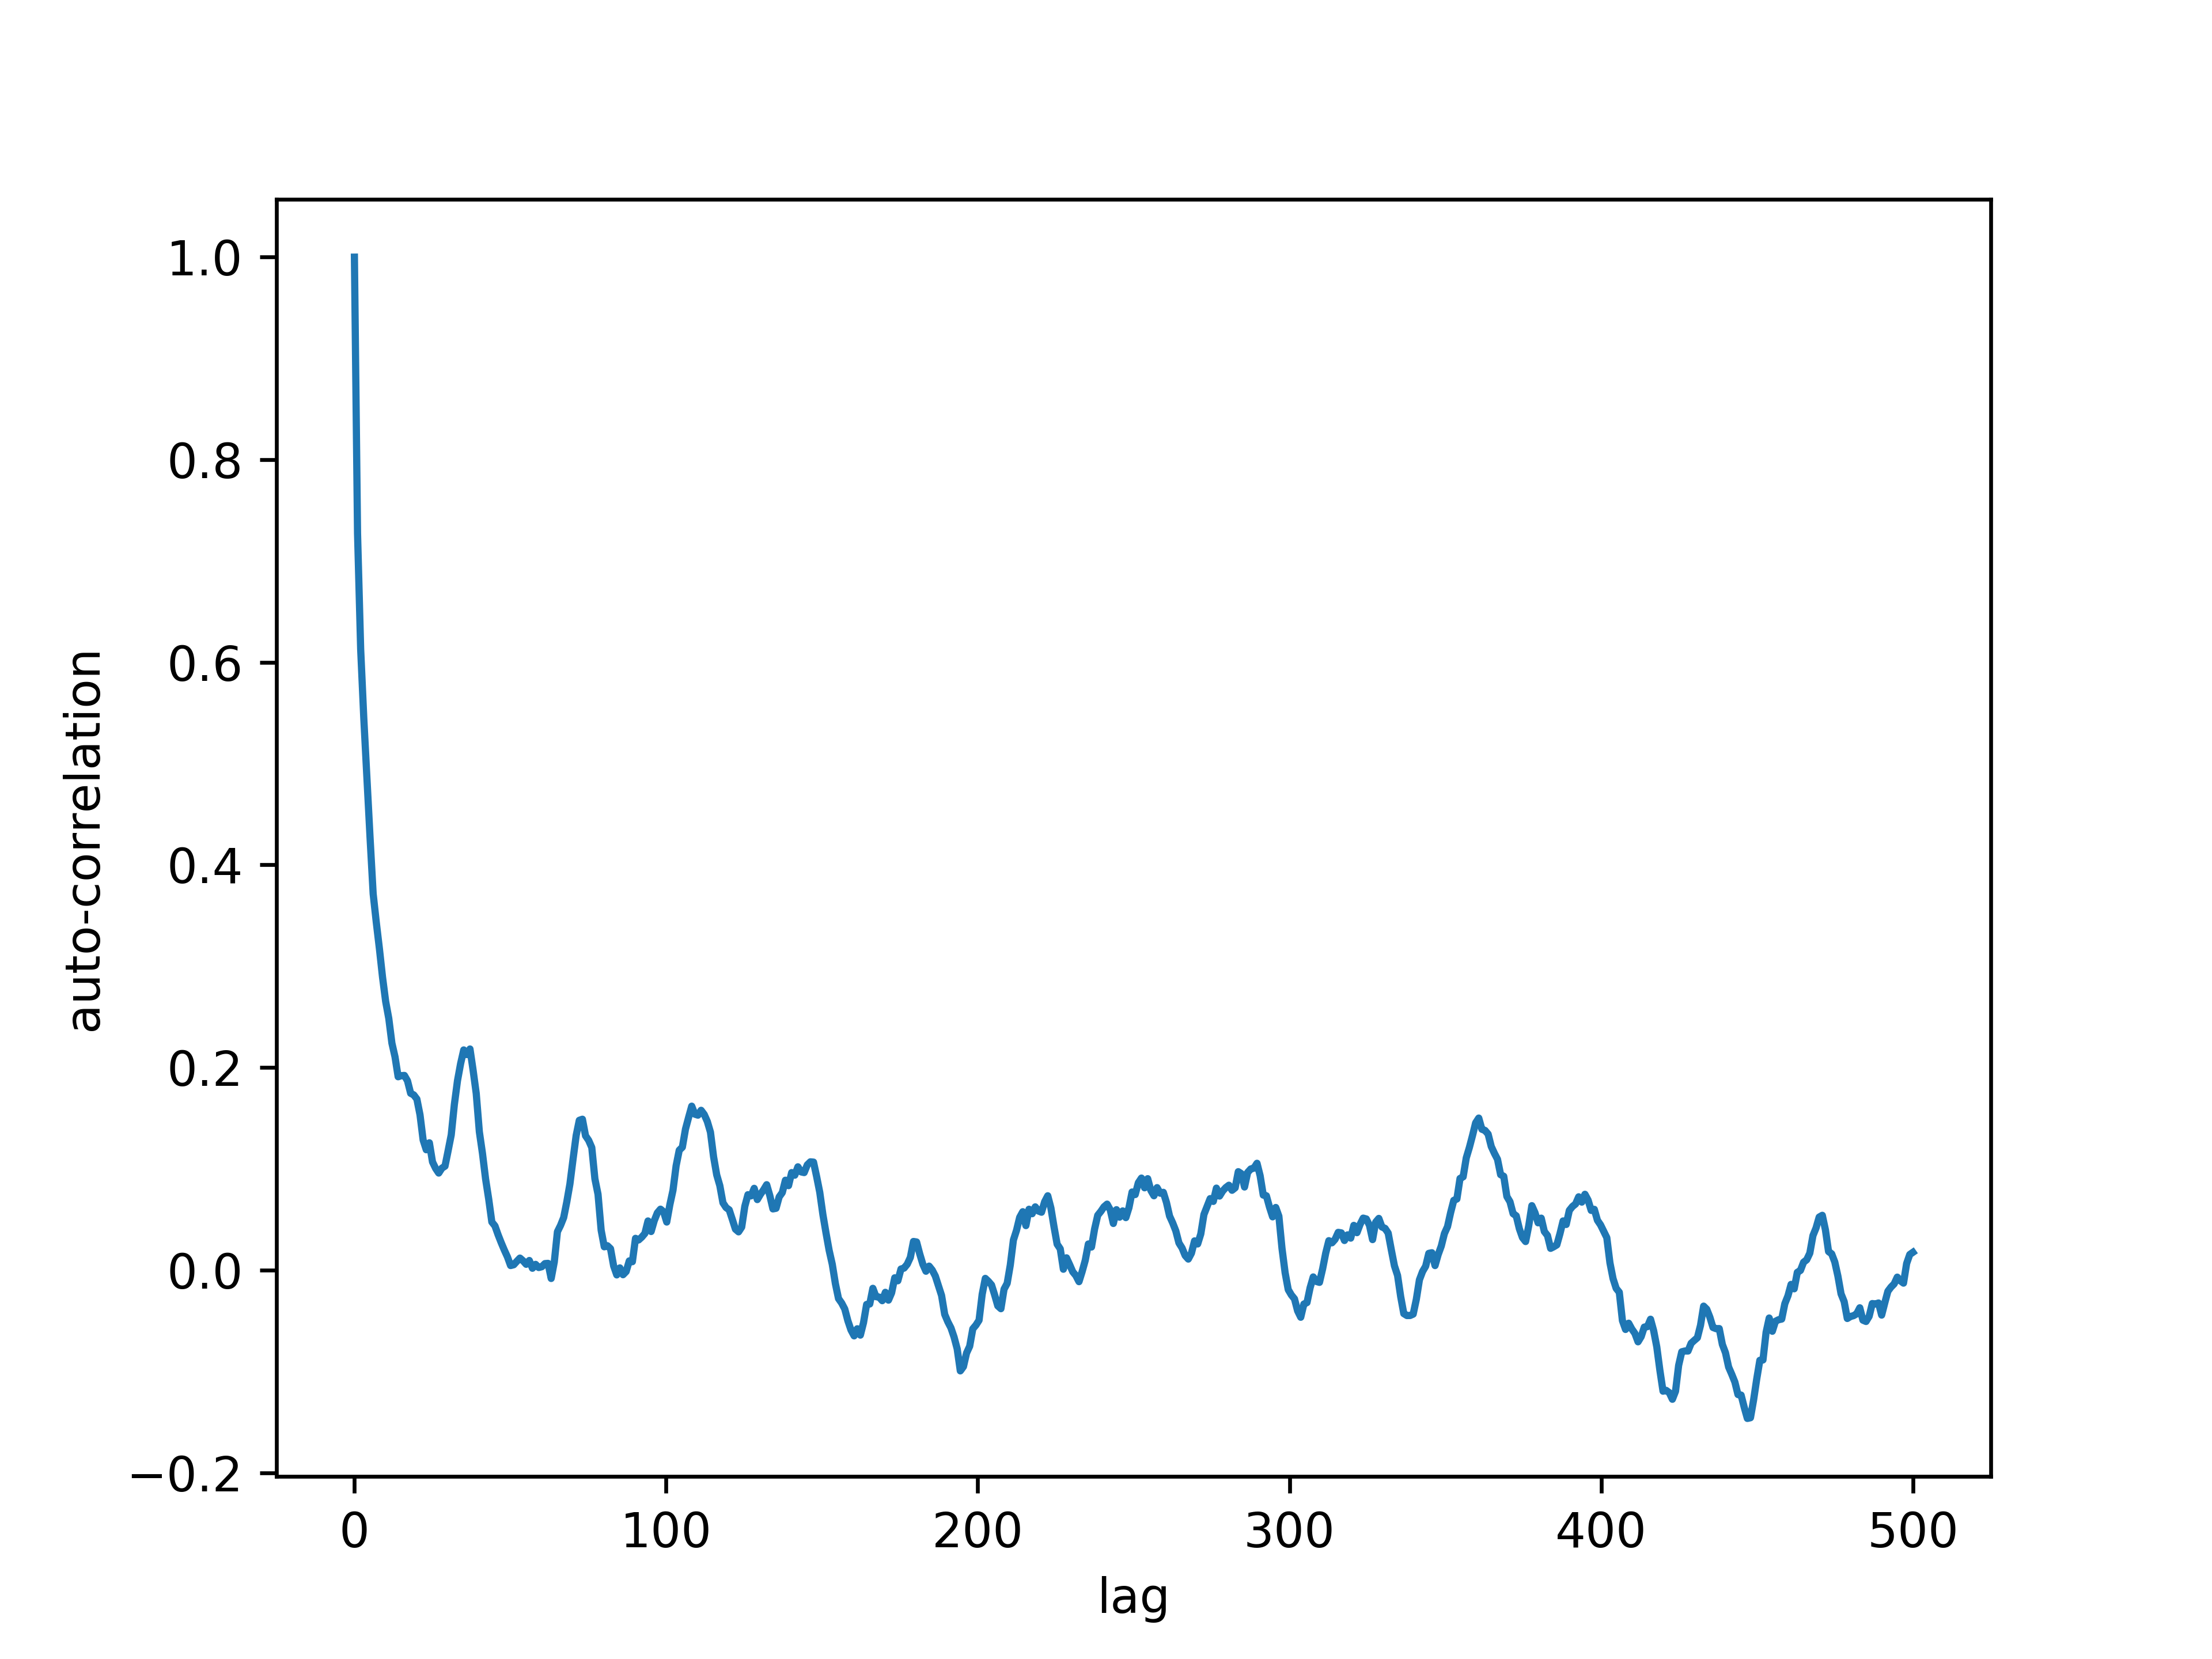
\includegraphics[width=0.9\textwidth]{figures/packet_count_correlation.png}
    \caption{Intensity auto-correlation as a function of lag}
    \label{fig:countcorr}
\end{figure}

\begin{figure}[H]
    \centering
    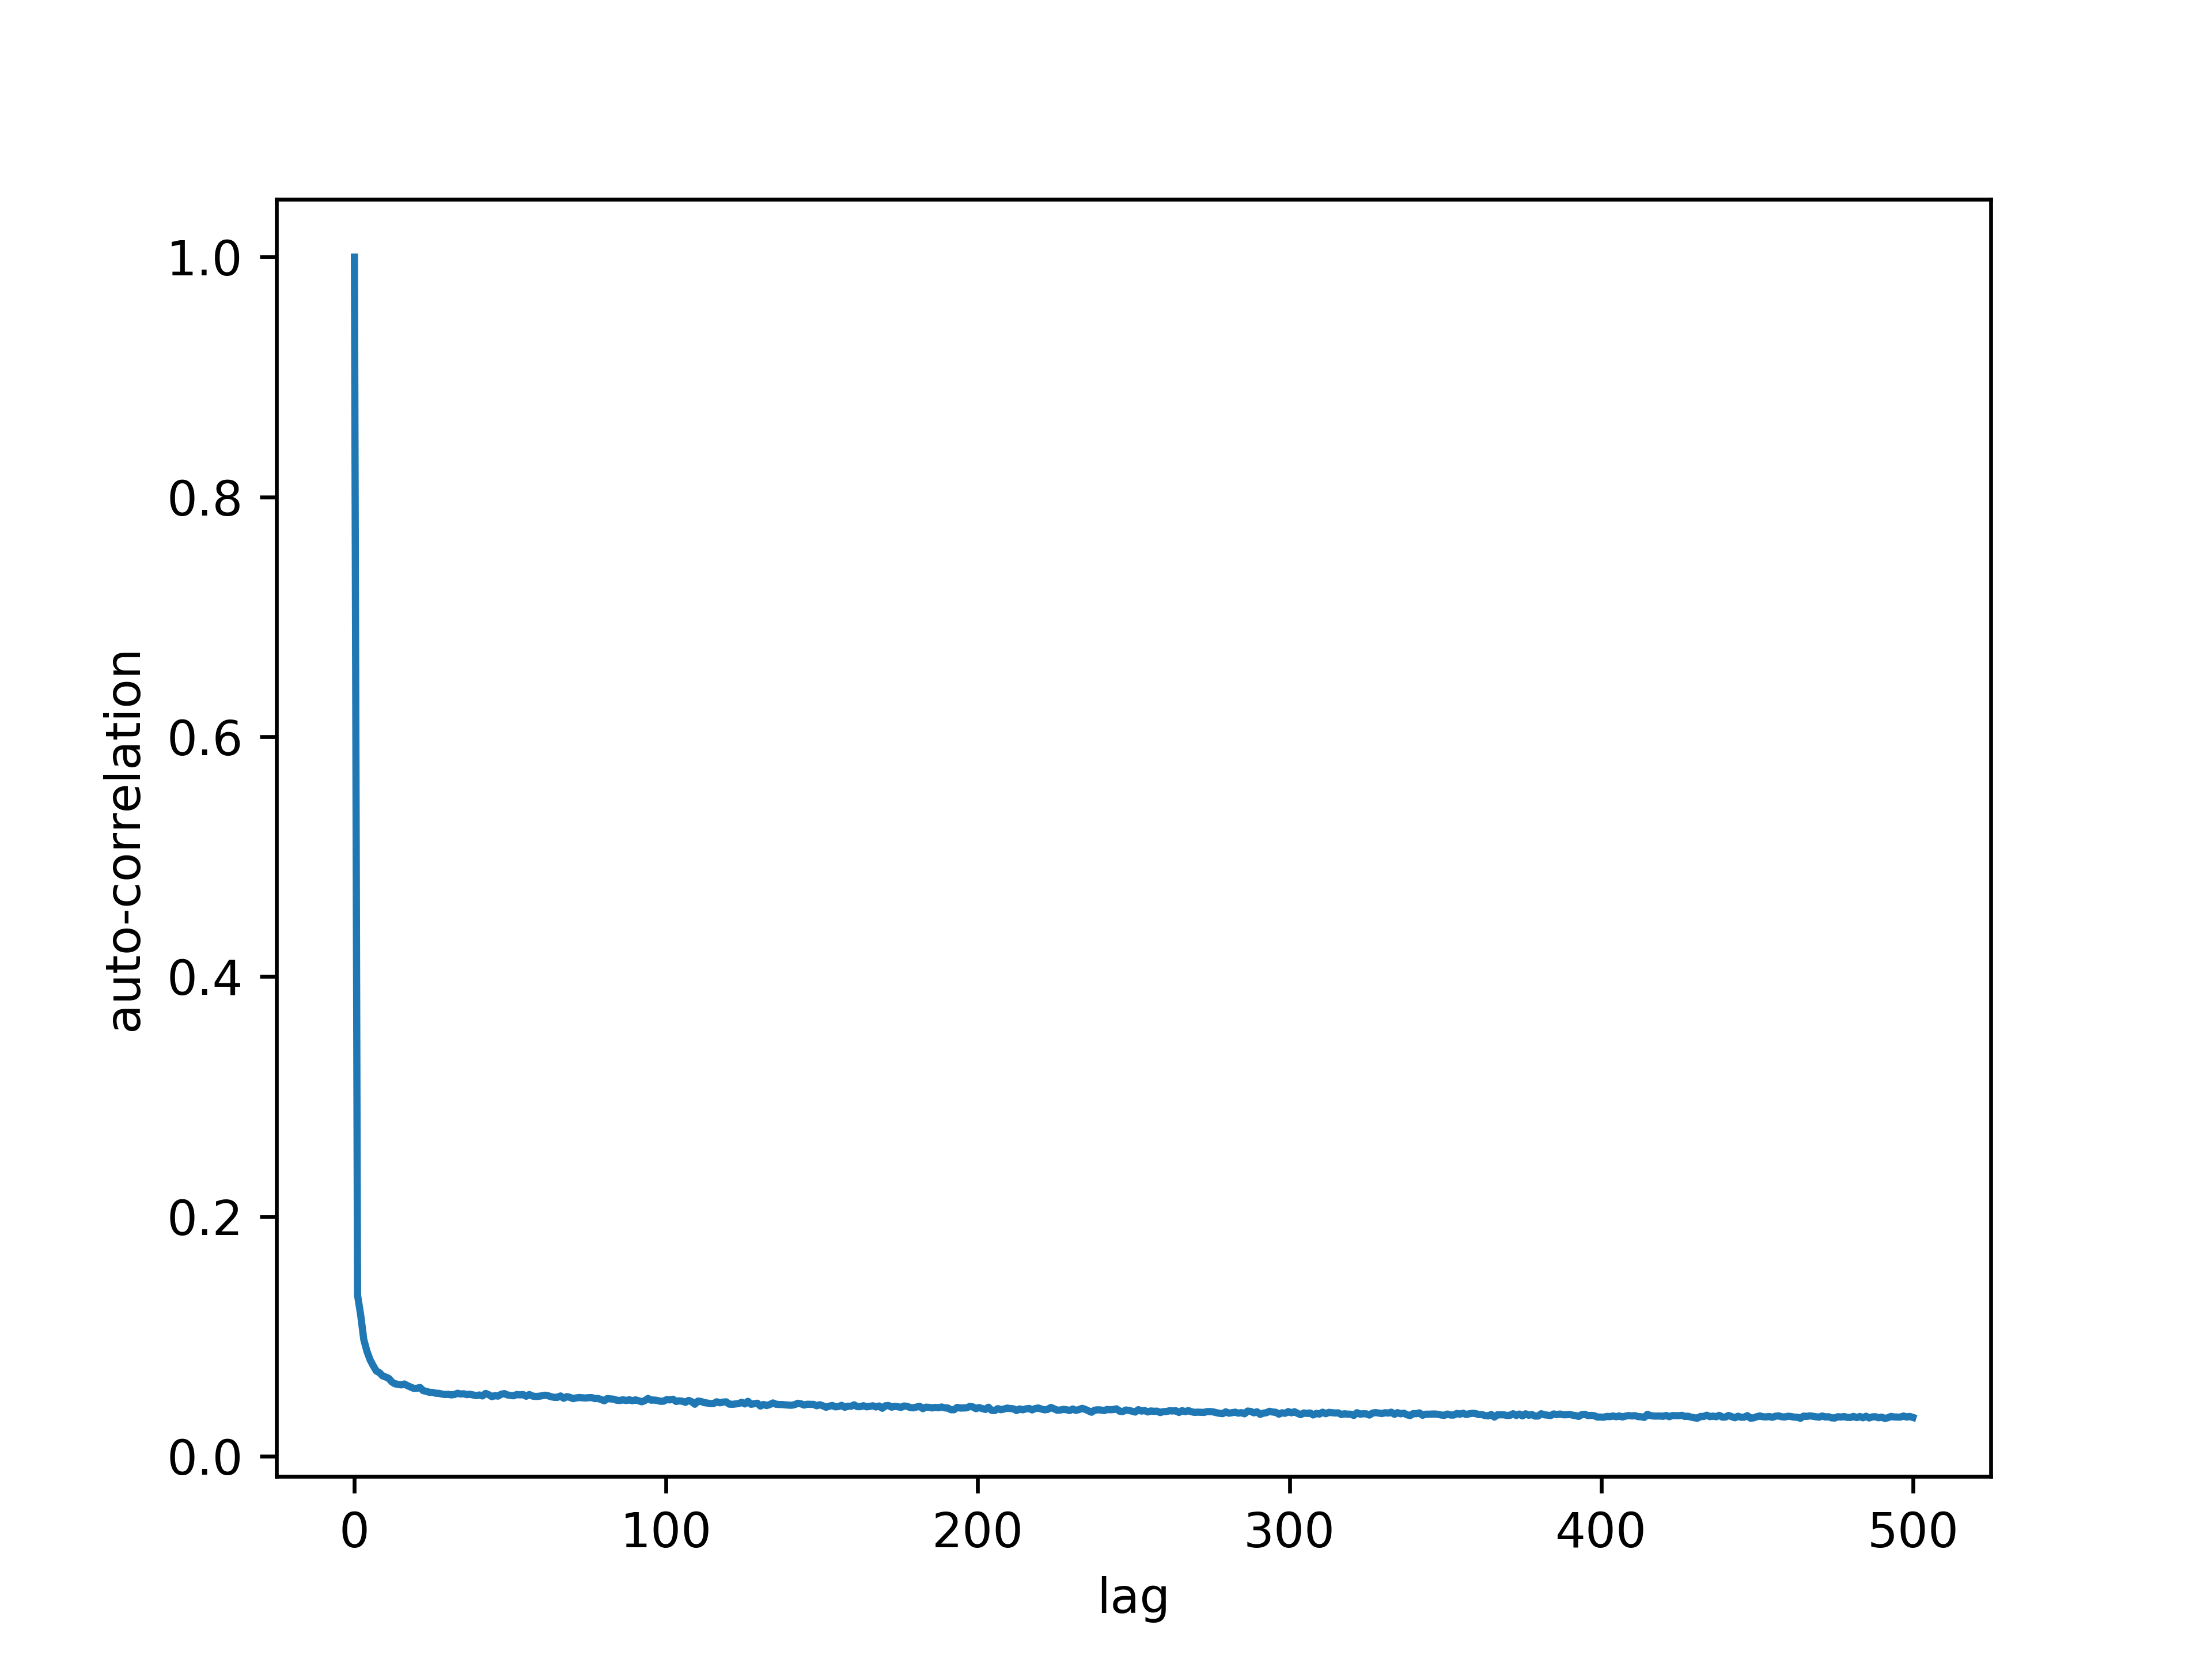
\includegraphics[width=0.9\textwidth]{figures/interarrival_correlation.png}
    \caption{Inter-arrival auto-correlation as a function of lag}
    \label{fig:interarrcorr}
\end{figure}

\subsection{IDI and IDC}

The \emph{Index of dispersion for Indices} (IDI) and \emph{Index of Dispersion for Counts} (IDC) were computationally intensive to calculate for the chosen data file.
For reducing the calculation times the code in Listing~\ref{lst:python} has been used that basically memoizes the windowed sum 
calculation for a given data set that can be reused when calculating IDI or IDC as a function of lag. The resulting plots can be seen of Figures \ref{fig:idi} and \ref{fig:idc}.

\begin{lstlisting}[style=mypython,caption={The functions used for calculating IDI and IDC},label={lst:python}]
windowed_sum_cache = {}

def get_windowed_sum(array, size):
    assert size > 0
    if (array.ctypes.data, size) not in windowed_sum_cache:
        if size == 1:
            windowed_sum_cache[(array.ctypes.data, size)] = array
        else:
            prev = get_windowed_sum(array, size - 1)
            wsum = np.fromiter((prev[i] + array[i + size - 1] for i in range(0, len(prev) - 1)), np.float64,
                               len(prev) - 1)
            windowed_sum_cache[(array.ctypes.data, size)] = wsum
    return windowed_sum_cache[(array.ctypes.data, size)]


def idi(interarrirval_times, lag):
    assert lag > 0
    return np.var(get_windowed_sum(interarrirval_times, lag)) / (
            lag * np.mean(interarrirval_times) * np.mean(interarrirval_times))

def idc(packet_counts, t):
    assert t > 0
    return np.var(get_windowed_sum(packet_counts, t)) / (t * np.mean(packet_counts))
\end{lstlisting}


\begin{figure}[H]
    \centering
    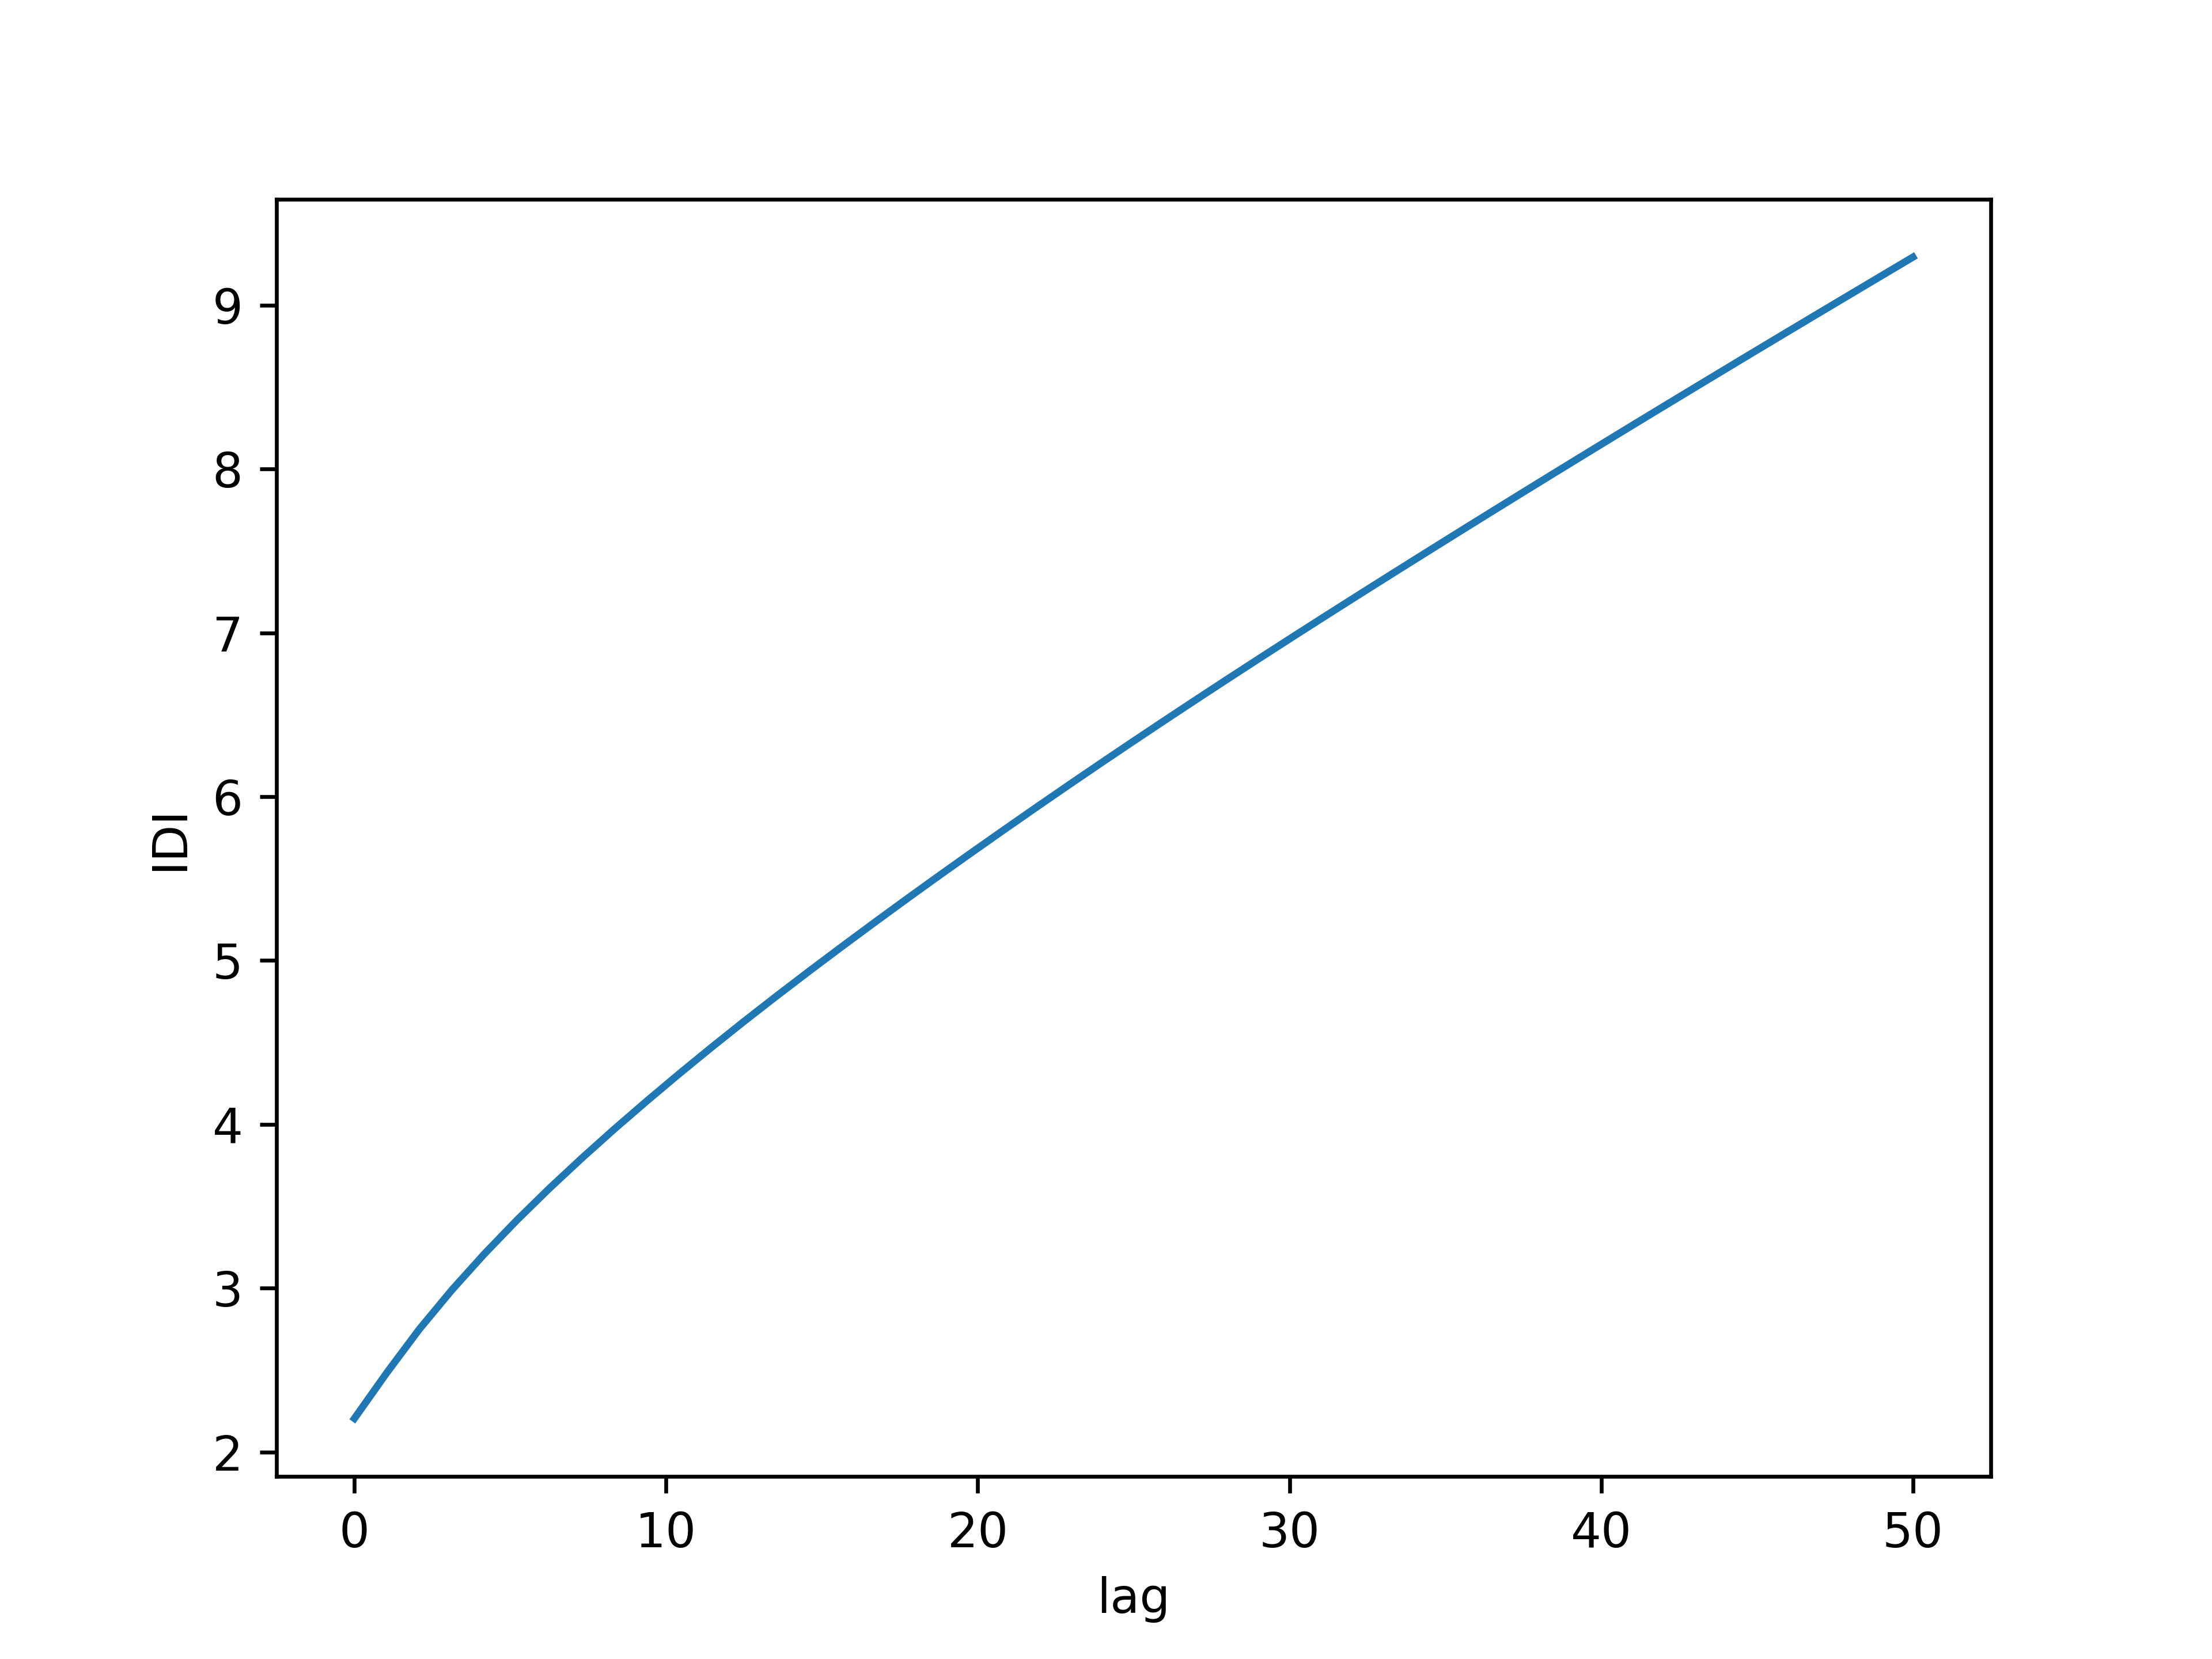
\includegraphics[width=0.9\textwidth]{figures/idi.png}
    \caption{Index of dispersion for Indices as function of lag}
    \label{fig:idi}
\end{figure}

\begin{figure}[H]
    \centering
    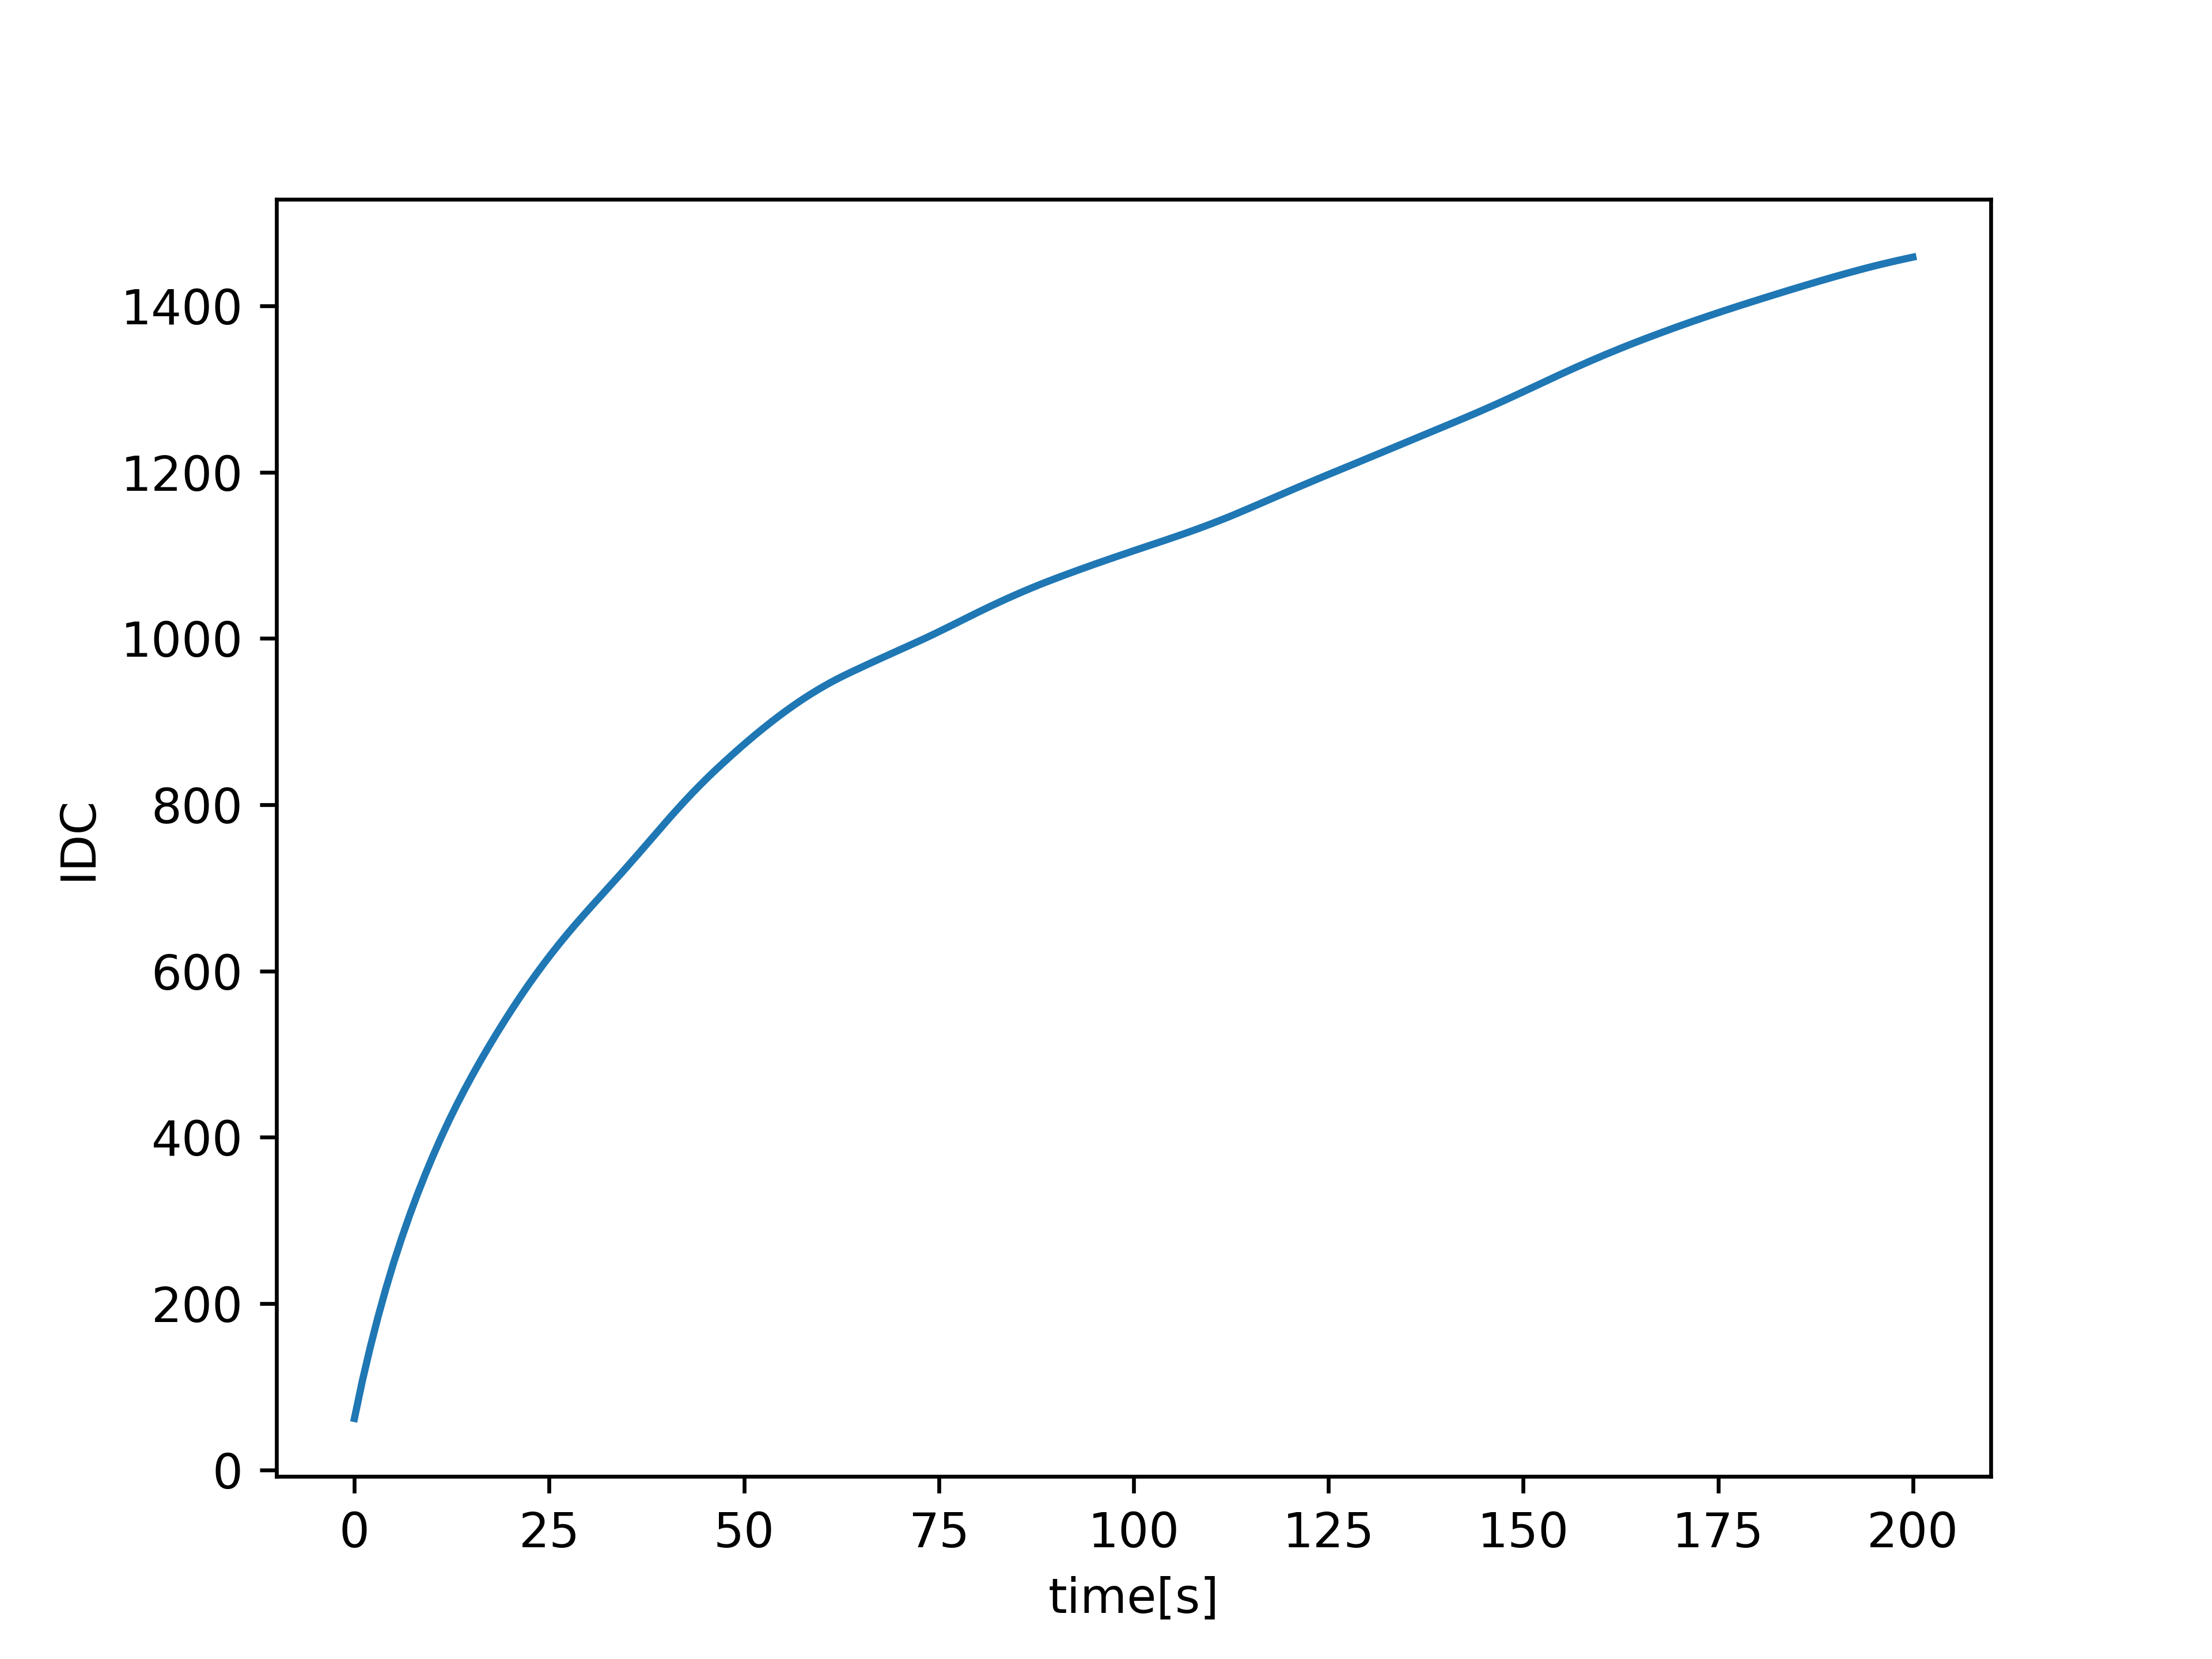
\includegraphics[width=0.9\textwidth]{figures/idc.png}
    \caption{Index of Dispersion for Counts as a function of lag}
    \label{fig:idc}
\end{figure}
	
	
\section{Conclusion}

As a part of this homework an arbitrarily chosen times series had to be analyzed similarly as presented in \cite{MolnarOnburst}. 
The selected data file contained data about 2.2 million TCP packets. The related statistics and statistical metrics and their plots and analysis have been presented.

\bibliographystyle{unsrt}
\bibliography{references}

\end{document}